\SourceLeaf{191}\par\noindent
\begin{minipage}[t]{.38\textwidth}
\vspace{0pt}
\centering
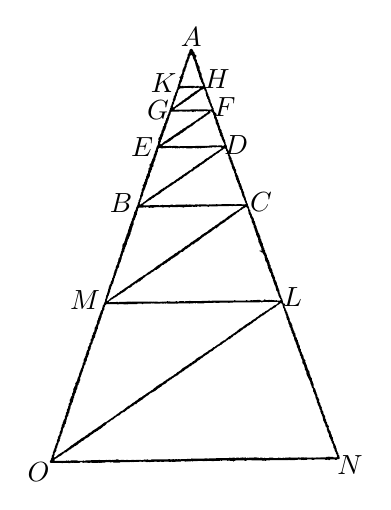
\begin{tikzpicture}[x=0.00441932cm,y=-0.00441932cm]
\fill[even odd rule] (480,91) -- (477,91) -- (475,92) -- (473,95) -- (473,98) -- (471,101) -- (471,103) -- (468,107) -- (468,113) -- (466,116) -- (465,121) -- (463,123) -- (462,127) -- (461,128) -- (461,133) -- (459,135) -- (459,139) -- (458,140) -- (458,142) -- (456,144) -- (456,146) -- (453,152) -- (452,161) -- (450,163) -- (450,165) -- (448,167) -- (448,169) -- (444,172) -- (444,173) -- (446,175) -- (446,178) -- (444,181) -- (443,187) -- (442,188) -- (442,191) -- (440,194) -- (440,198) -- (438,202) -- (438,205) -- (436,208) -- (435,213) -- (432,217) -- (431,223) -- (428,227) -- (427,233) -- (425,236) -- (425,242) -- (423,244) -- (423,247) -- (422,248) -- (421,253) -- (419,255) -- (419,259) -- (417,262) -- (417,265) -- (415,267) -- (415,271) -- (413,273) -- (413,276) -- (412,277) -- (412,279) -- (410,281) -- (409,287) -- (406,291) -- (406,294) -- (404,297) -- (403,303) -- (400,306) -- (400,311) -- (397,314) -- (395,323) -- (393,325) -- (393,327) -- (392,328) -- (392,332) -- (390,336) -- (388,338) -- (388,342) -- (386,344) -- (384,348) -- (384,352) -- (385,354) -- (383,357) -- (383,362) -- (382,363) -- (382,366) -- (381,367) -- (381,369) -- (379,371) -- (376,382) -- (374,385) -- (373,391) -- (371,394) -- (369,403) -- (366,408) -- (366,410) -- (364,413) -- (363,418) -- (358,423) -- (359,429) -- (357,433) -- (355,435) -- (356,438) -- (354,442) -- (354,447) -- (351,450) -- (351,454) -- (349,456) -- (348,463) -- (346,465) -- (345,471) -- (343,473) -- (343,475) -- (342,476) -- (342,479) -- (338,482) -- (340,484) -- (340,485) -- (339,486) -- (339,489) -- (336,495) -- (336,501) -- (334,503) -- (333,509) -- (331,512) -- (331,518) -- (329,521) -- (329,523) -- (327,525) -- (327,530) -- (325,533) -- (324,539) -- (320,547) -- (319,552) -- (316,558) -- (314,560) -- (314,565) -- (313,566) -- (311,574) -- (308,579) -- (308,582) -- (305,588) -- (304,593) -- (302,595) -- (302,599) -- (300,601) -- (300,605) -- (298,608) -- (295,620) -- (292,625) -- (292,628) -- (290,631) -- (290,634) -- (288,637) -- (288,640) -- (286,643) -- (286,646) -- (281,652) -- (281,655) -- (280,656) -- (281,661) -- (280,662) -- (280,665) -- (278,667) -- (278,671) -- (276,674) -- (276,677) -- (273,684) -- (273,688) -- (269,693) -- (269,698) -- (268,699) -- (268,702) -- (266,704) -- (266,708) -- (262,715) -- (262,717) -- (261,718) -- (261,722) -- (258,727) -- (257,733) -- (255,736) -- (255,741) -- (254,742) -- (253,747) -- (251,749) -- (251,754) -- (249,756) -- (247,760) -- (247,764) -- (243,769) -- (243,772) -- (241,774) -- (242,777) -- (240,780) -- (239,786) -- (238,787) -- (238,790) -- (237,791) -- (236,796) -- (234,799) -- (234,802) -- (233,803) -- (233,806) -- (231,810) -- (231,814) -- (230,815) -- (230,817) -- (228,820) -- (227,824) -- (224,828) -- (224,832) -- (222,835) -- (222,839) -- (220,841) -- (217,847) -- (217,849) -- (215,852) -- (215,855) -- (213,857) -- (212,863) -- (211,864) -- (211,867) -- (209,869) -- (209,872) -- (207,874) -- (208,878) -- (206,882) -- (204,884) -- (204,887) -- (201,891) -- (200,901) -- (196,907) -- (196,910) -- (195,912) -- (193,914) -- (193,919) -- (192,920) -- (192,922) -- (189,925) -- (189,933) -- (186,936) -- (186,940) -- (185,941) -- (185,943) -- (183,945) -- (181,949) -- (182,953) -- (179,956) -- (179,958) -- (177,961) -- (177,964) -- (175,968) -- (175,972) -- (173,974) -- (173,976) -- (169,984) -- (169,990) -- (166,994) -- (166,999) -- (165,1000) -- (164,1005) -- (162,1008) -- (162,1010) -- (160,1012) -- (160,1016) -- (158,1018) -- (158,1020) -- (156,1024) -- (156,1028) -- (155,1029) -- (155,1031) -- (153,1033) -- (150,1044) -- (145,1051) -- (146,1055) -- (144,1059) -- (142,1061) -- (142,1064) -- (139,1067) -- (140,1069) -- (140,1072) -- (139,1073) -- (139,1076) -- (136,1080) -- (136,1083) -- (137,1085) -- (134,1088) -- (132,1092) -- (132,1094) -- (130,1096) -- (130,1099) -- (129,1100) -- (130,1105) -- (126,1110) -- (126,1116) -- (125,1117) -- (124,1122) -- (121,1127) -- (121,1132) -- (118,1136) -- (118,1141) -- (115,1147) -- (116,1150) -- (111,1158) -- (111,1160) -- (109,1164) -- (109,1167) -- (107,1169) -- (107,1171) -- (106,1172) -- (106,1176) -- (104,1180) -- (104,1185) -- (102,1187) -- (102,1189) -- (100,1192) -- (100,1197) -- (95,1206) -- (95,1211) -- (93,1213) -- (92,1221) -- (89,1226) -- (89,1228) -- (87,1232) -- (87,1235) -- (85,1237) -- (85,1240) -- (83,1242) -- (83,1246) -- (81,1248) -- (81,1254) -- (78,1258) -- (78,1261) -- (77,1262) -- (77,1265) -- (75,1268) -- (75,1271) -- (72,1274) -- (72,1277) -- (75,1279) -- (106,1279) -- (107,1280) -- (109,1280) -- (110,1279) -- (125,1279) -- (126,1280) -- (130,1280) -- (133,1278) -- (135,1279) -- (139,1279) -- (140,1278) -- (142,1279) -- (157,1279) -- (160,1277) -- (165,1277) -- (168,1279) -- (170,1278) -- (180,1278) -- (181,1279) -- (187,1279) -- (188,1278) -- (192,1278) -- (193,1279) -- (211,1279) -- (213,1278) -- (214,1279) -- (217,1279) -- (219,1278) -- (221,1279) -- (222,1278) -- (231,1278) -- (232,1277) -- (246,1277) -- (247,1278) -- (249,1277) -- (254,1277) -- (255,1278) -- (273,1278) -- (274,1277) -- (302,1277) -- (303,1276) -- (306,1276) -- (307,1277) -- (311,1276) -- (313,1277) -- (314,1276) -- (328,1276) -- (329,1275) -- (335,1275) -- (336,1276) -- (346,1275) -- (349,1277) -- (351,1276) -- (353,1277) -- (355,1276) -- (360,1277) -- (361,1276) -- (371,1276) -- (372,1275) -- (379,1275) -- (380,1276) -- (387,1276) -- (388,1275) -- (392,1275) -- (393,1276) -- (399,1276) -- (400,1275) -- (413,1275) -- (414,1276) -- (419,1276) -- (420,1275) -- (422,1275) -- (423,1276) -- (432,1276) -- (433,1275) -- (448,1275) -- (450,1273) -- (452,1274) -- (459,1274) -- (460,1275) -- (464,1275) -- (465,1274) -- (467,1274) -- (468,1275) -- (480,1274) -- (482,1275) -- (483,1274) -- (496,1274) -- (497,1273) -- (510,1273) -- (511,1274) -- (516,1274) -- (517,1273) -- (519,1273) -- (520,1274) -- (522,1274) -- (523,1273) -- (536,1273) -- (537,1274) -- (543,1274) -- (544,1273) -- (560,1273) -- (561,1272) -- (563,1272) -- (564,1273) -- (566,1273) -- (567,1272) -- (581,1272) -- (582,1273) -- (589,1272) -- (590,1273) -- (597,1273) -- (599,1275) -- (600,1275) -- (602,1273) -- (604,1273) -- (605,1272) -- (627,1272) -- (628,1271) -- (632,1273) -- (635,1273) -- (638,1271) -- (651,1271) -- (652,1272) -- (682,1272) -- (683,1273) -- (689,1272) -- (690,1273) -- (692,1273) -- (693,1272) -- (696,1272) -- (697,1271) -- (699,1272) -- (703,1272) -- (704,1271) -- (757,1271) -- (758,1270) -- (760,1271) -- (776,1271) -- (777,1270) -- (783,1270) -- (784,1269) -- (794,1270) -- (795,1271) -- (797,1270) -- (802,1271) -- (803,1270) -- (810,1270) -- (811,1269) -- (823,1269) -- (824,1270) -- (831,1270) -- (832,1269) -- (858,1269) -- (859,1268) -- (863,1270) -- (868,1270) -- (870,1269) -- (873,1271) -- (875,1271) -- (877,1269) -- (890,1269) -- (891,1270) -- (895,1270) -- (898,1268) -- (902,1268) -- (904,1266) -- (903,1258) -- (900,1255) -- (900,1251) -- (898,1249) -- (898,1247) -- (896,1245) -- (896,1242) -- (895,1241) -- (895,1237) -- (894,1236) -- (893,1230) -- (891,1228) -- (891,1226) -- (888,1222) -- (887,1217) -- (885,1215) -- (885,1211) -- (884,1210) -- (885,1207) -- (882,1203) -- (881,1198) -- (879,1195) -- (878,1189) -- (875,1186) -- (875,1184) -- (873,1182) -- (873,1180) -- (872,1179) -- (873,1174) -- (868,1167) -- (868,1163) -- (866,1161) -- (865,1159) -- (865,1155) -- (862,1151) -- (862,1145) -- (861,1144) -- (861,1142) -- (859,1140) -- (857,1136) -- (857,1132) -- (854,1128) -- (854,1125) -- (852,1122) -- (853,1119) -- (851,1117) -- (849,1113) -- (849,1110) -- (847,1106) -- (845,1104) -- (845,1100) -- (846,1098) -- (844,1096) -- (843,1092) -- (840,1089) -- (840,1084) -- (838,1081) -- (838,1078) -- (836,1076) -- (836,1072) -- (834,1070) -- (834,1067) -- (829,1061) -- (829,1052) -- (827,1049) -- (827,1047) -- (824,1041) -- (824,1036) -- (822,1034) -- (820,1030) -- (820,1028) -- (818,1024) -- (817,1016) -- (815,1014) -- (812,1008) -- (809,997) -- (807,995) -- (807,992) -- (805,989) -- (806,985) -- (801,979) -- (800,972) -- (796,965) -- (795,961) -- (793,959) -- (793,953) -- (790,950) -- (790,944) -- (788,940) -- (786,938) -- (786,934) -- (784,931) -- (784,927) -- (781,924) -- (781,920) -- (778,917) -- (778,912) -- (777,911) -- (777,908) -- (774,905) -- (774,901) -- (772,899) -- (770,892) -- (768,889) -- (768,883) -- (766,881) -- (766,878) -- (764,876) -- (760,869) -- (761,866) -- (759,863) -- (759,861) -- (757,858) -- (756,853) -- (754,850) -- (754,847) -- (751,844) -- (751,841) -- (749,839) -- (749,836) -- (746,832) -- (746,829) -- (745,827) -- (747,825) -- (748,825) -- (747,824) -- (747,822) -- (744,822) -- (742,820) -- (739,808) -- (737,806) -- (736,800) -- (734,798) -- (734,795) -- (732,792) -- (732,789) -- (731,788) -- (731,783) -- (729,781) -- (729,778) -- (727,775) -- (727,772) -- (725,769) -- (723,760) -- (721,758) -- (721,756) -- (719,754) -- (718,746) -- (716,743) -- (716,741) -- (714,739) -- (714,736) -- (711,730) -- (711,726) -- (709,723) -- (709,721) -- (706,718) -- (706,712) -- (703,709) -- (703,704) -- (702,703) -- (701,698) -- (699,696) -- (698,692) -- (695,687) -- (695,682) -- (693,680) -- (693,677) -- (690,674) -- (690,669) -- (688,667) -- (688,664) -- (686,662) -- (686,659) -- (684,656) -- (684,651) -- (680,644) -- (679,638) -- (677,636) -- (676,628) -- (674,625) -- (673,621) -- (670,617) -- (670,614) -- (668,611) -- (668,609) -- (666,605) -- (666,602) -- (662,594) -- (662,590) -- (661,589) -- (661,587) -- (658,583) -- (658,579) -- (652,569) -- (652,567) -- (648,559) -- (648,555) -- (646,553) -- (644,549) -- (644,546) -- (641,540) -- (640,535) -- (638,532) -- (638,530) -- (635,523) -- (634,517) -- (631,512) -- (631,509) -- (630,508) -- (630,503) -- (626,496) -- (626,493) -- (624,491) -- (624,487) -- (623,486) -- (623,484) -- (621,482) -- (621,478) -- (618,475) -- (618,470) -- (616,468) -- (615,463) -- (613,460) -- (613,457) -- (610,452) -- (610,450) -- (607,446) -- (607,438) -- (603,433) -- (603,430) -- (600,425) -- (600,422) -- (597,416) -- (597,412) -- (594,409) -- (594,405) -- (590,398) -- (590,396) -- (588,394) -- (588,389) -- (590,388) -- (590,386) -- (589,384) -- (587,385) -- (584,382) -- (581,376) -- (580,369) -- (577,364) -- (577,360) -- (575,356) -- (575,353) -- (572,348) -- (572,345) -- (570,343) -- (570,340) -- (568,338) -- (568,333) -- (565,329) -- (565,324) -- (561,319) -- (561,315) -- (558,309) -- (558,305) -- (555,301) -- (555,295) -- (552,292) -- (551,287) -- (549,284) -- (549,281) -- (551,279) -- (550,276) -- (549,276) -- (544,271) -- (544,269) -- (542,265) -- (542,261) -- (540,259) -- (540,257) -- (538,255) -- (537,249) -- (534,244) -- (533,237) -- (531,235) -- (531,231) -- (529,227) -- (527,225) -- (527,221) -- (525,218) -- (525,216) -- (524,215) -- (524,213) -- (521,206) -- (521,203) -- (518,199) -- (518,196) -- (517,195) -- (516,190) -- (513,185) -- (512,179) -- (508,170) -- (508,163) -- (506,159) -- (504,157) -- (504,153) -- (502,151) -- (502,142) -- (499,139) -- (499,137) -- (497,135) -- (497,132) -- (495,130) -- (495,128) -- (494,127) -- (494,123) -- (491,119) -- (491,116) -- (492,115) -- (493,110) -- (488,106) -- (488,102) -- (484,98) -- (483,94) -- cycle
(897,1259) -- (897,1261) -- (895,1263) -- (886,1263) -- (885,1262) -- (875,1262) -- (874,1261) -- (872,1261) -- (871,1262) -- (866,1262) -- (865,1263) -- (849,1263) -- (848,1264) -- (846,1264) -- (845,1263) -- (843,1264) -- (841,1264) -- (840,1263) -- (838,1263) -- (837,1264) -- (826,1264) -- (825,1263) -- (823,1264) -- (810,1264) -- (809,1263) -- (806,1263) -- (805,1264) -- (803,1264) -- (802,1263) -- (794,1263) -- (793,1264) -- (789,1264) -- (788,1263) -- (785,1263) -- (784,1264) -- (763,1264) -- (762,1263) -- (759,1263) -- (758,1264) -- (747,1264) -- (746,1265) -- (744,1265) -- (743,1264) -- (741,1264) -- (740,1265) -- (735,1265) -- (734,1264) -- (732,1265) -- (730,1264) -- (728,1264) -- (727,1265) -- (714,1265) -- (713,1264) -- (702,1264) -- (701,1265) -- (690,1265) -- (689,1264) -- (687,1265) -- (683,1265) -- (682,1264) -- (676,1264) -- (675,1265) -- (672,1265) -- (671,1264) -- (666,1264) -- (665,1263) -- (659,1263) -- (658,1264) -- (644,1264) -- (643,1265) -- (639,1264) -- (638,1265) -- (636,1265) -- (634,1263) -- (632,1264) -- (627,1264) -- (625,1263) -- (624,1264) -- (619,1264) -- (618,1265) -- (616,1265) -- (615,1264) -- (608,1264) -- (607,1265) -- (603,1265) -- (602,1264) -- (597,1264) -- (596,1265) -- (588,1264) -- (587,1265) -- (550,1265) -- (549,1266) -- (529,1266) -- (528,1267) -- (525,1267) -- (524,1266) -- (517,1266) -- (516,1267) -- (482,1267) -- (480,1266) -- (476,1268) -- (468,1267) -- (467,1268) -- (449,1268) -- (448,1269) -- (445,1269) -- (444,1268) -- (440,1268) -- (439,1269) -- (437,1269) -- (436,1268) -- (433,1268) -- (432,1269) -- (429,1269) -- (428,1268) -- (425,1268) -- (424,1269) -- (417,1269) -- (416,1268) -- (413,1268) -- (412,1269) -- (364,1269) -- (363,1270) -- (354,1270) -- (353,1269) -- (346,1270) -- (344,1269) -- (343,1270) -- (339,1270) -- (338,1271) -- (334,1271) -- (333,1270) -- (319,1270) -- (318,1271) -- (315,1271) -- (314,1270) -- (307,1270) -- (306,1271) -- (297,1271) -- (296,1270) -- (292,1270) -- (291,1271) -- (286,1271) -- (285,1270) -- (276,1270) -- (275,1271) -- (272,1271) -- (268,1269) -- (263,1269) -- (262,1270) -- (255,1270) -- (254,1271) -- (252,1270) -- (250,1271) -- (247,1271) -- (246,1270) -- (241,1270) -- (240,1271) -- (237,1271) -- (236,1270) -- (234,1270) -- (233,1271) -- (216,1271) -- (215,1270) -- (213,1270) -- (212,1271) -- (191,1271) -- (190,1272) -- (175,1272) -- (174,1273) -- (170,1273) -- (169,1272) -- (167,1273) -- (152,1273) -- (151,1272) -- (133,1272) -- (132,1273) -- (127,1273) -- (125,1272) -- (124,1273) -- (122,1273) -- (120,1272) -- (119,1273) -- (91,1273) -- (89,1274) -- (85,1272) -- (85,1270) -- (88,1267) -- (93,1265) -- (96,1262) -- (104,1258) -- (115,1249) -- (118,1249) -- (120,1248) -- (124,1244) -- (125,1244) -- (130,1240) -- (132,1240) -- (137,1235) -- (139,1235) -- (143,1231) -- (147,1230) -- (149,1228) -- (150,1228) -- (156,1222) -- (160,1220) -- (164,1216) -- (167,1216) -- (173,1210) -- (183,1205) -- (188,1200) -- (196,1195) -- (199,1192) -- (204,1190) -- (206,1188) -- (209,1187) -- (212,1184) -- (218,1181) -- (227,1173) -- (230,1172) -- (238,1163) -- (241,1163) -- (249,1156) -- (251,1156) -- (253,1154) -- (254,1154) -- (259,1149) -- (262,1148) -- (265,1145) -- (269,1143) -- (271,1143) -- (278,1136) -- (284,1133) -- (286,1133) -- (295,1125) -- (296,1125) -- (298,1123) -- (300,1123) -- (305,1118) -- (311,1115) -- (315,1111) -- (317,1110) -- (321,1110) -- (321,1109) -- (326,1104) -- (329,1103) -- (334,1099) -- (337,1098) -- (343,1092) -- (344,1092) -- (351,1086) -- (353,1086) -- (359,1080) -- (375,1072) -- (383,1065) -- (386,1064) -- (389,1061) -- (392,1060) -- (395,1056) -- (405,1051) -- (411,1044) -- (413,1044) -- (418,1040) -- (421,1039) -- (425,1035) -- (426,1035) -- (431,1031) -- (433,1031) -- (435,1029) -- (438,1028) -- (447,1020) -- (449,1020) -- (453,1016) -- (455,1016) -- (463,1009) -- (468,1007) -- (473,1002) -- (477,1001) -- (482,996) -- (484,996) -- (486,994) -- (493,990) -- (497,985) -- (499,985) -- (501,983) -- (502,983) -- (506,979) -- (509,978) -- (514,973) -- (517,972) -- (519,970) -- (526,966) -- (531,961) -- (535,959) -- (537,959) -- (547,950) -- (550,949) -- (554,945) -- (560,942) -- (562,940) -- (564,940) -- (572,933) -- (575,932) -- (579,928) -- (582,927) -- (585,924) -- (588,924) -- (593,919) -- (595,919) -- (600,913) -- (604,912) -- (614,904) -- (616,904) -- (621,899) -- (623,899) -- (629,893) -- (631,893) -- (633,891) -- (634,891) -- (640,885) -- (642,885) -- (646,883) -- (649,880) -- (653,878) -- (658,873) -- (664,870) -- (670,864) -- (673,863) -- (682,856) -- (684,856) -- (687,853) -- (689,853) -- (694,848) -- (698,846) -- (706,839) -- (709,839) -- (715,834) -- (719,833) -- (724,827) -- (727,826) -- (735,820) -- (736,820) -- (739,823) -- (740,825) -- (740,828) -- (742,831) -- (742,834) -- (745,838) -- (745,842) -- (747,845) -- (747,848) -- (749,851) -- (749,854) -- (751,857) -- (751,862) -- (752,863) -- (753,868) -- (756,871) -- (757,879) -- (760,884) -- (760,888) -- (763,892) -- (763,895) -- (766,901) -- (766,905) -- (770,910) -- (770,914) -- (773,919) -- (774,926) -- (778,933) -- (778,935) -- (781,942) -- (781,945) -- (785,953) -- (786,958) -- (789,963) -- (789,965) -- (790,966) -- (790,970) -- (793,973) -- (793,977) -- (797,985) -- (797,992) -- (802,999) -- (803,1005) -- (804,1006) -- (804,1011) -- (808,1016) -- (809,1025) -- (820,1047) -- (820,1051) -- (823,1057) -- (824,1062) -- (827,1065) -- (827,1067) -- (828,1068) -- (828,1074) -- (830,1076) -- (830,1078) -- (834,1086) -- (835,1093) -- (836,1094) -- (836,1096) -- (838,1098) -- (839,1106) -- (841,1108) -- (841,1111) -- (846,1121) -- (846,1124) -- (849,1128) -- (849,1133) -- (851,1135) -- (851,1138) -- (853,1140) -- (853,1143) -- (855,1146) -- (857,1157) -- (863,1169) -- (863,1173) -- (867,1178) -- (867,1184) -- (869,1186) -- (869,1189) -- (873,1196) -- (874,1204) -- (876,1206) -- (876,1208) -- (878,1210) -- (878,1213) -- (881,1217) -- (881,1220) -- (885,1226) -- (885,1229) -- (886,1230) -- (886,1235) -- (889,1239) -- (890,1244) -- (893,1249) -- (893,1252) -- (895,1254) -- (895,1256) -- cycle
(728,817) -- (728,819) -- (724,824) -- (722,824) -- (720,826) -- (716,827) -- (709,833) -- (707,833) -- (697,841) -- (692,843) -- (686,848) -- (684,848) -- (679,853) -- (676,853) -- (670,859) -- (666,861) -- (663,864) -- (654,869) -- (647,875) -- (645,875) -- (643,877) -- (633,883) -- (625,890) -- (622,891) -- (620,893) -- (618,893) -- (607,903) -- (606,903) -- (603,906) -- (600,907) -- (597,910) -- (594,911) -- (590,915) -- (588,915) -- (574,927) -- (570,928) -- (568,930) -- (564,932) -- (558,938) -- (553,940) -- (544,947) -- (542,947) -- (535,953) -- (527,957) -- (523,961) -- (520,962) -- (518,964) -- (514,966) -- (509,971) -- (507,971) -- (504,974) -- (502,974) -- (494,979) -- (486,987) -- (484,987) -- (480,991) -- (475,993) -- (469,998) -- (454,1007) -- (446,1015) -- (444,1015) -- (442,1017) -- (439,1018) -- (433,1024) -- (430,1025) -- (426,1029) -- (423,1030) -- (420,1033) -- (416,1034) -- (410,1039) -- (407,1040) -- (404,1043) -- (400,1045) -- (396,1049) -- (395,1049) -- (393,1051) -- (391,1051) -- (389,1053) -- (386,1054) -- (384,1056) -- (380,1058) -- (376,1062) -- (372,1064) -- (366,1070) -- (363,1071) -- (361,1073) -- (348,1081) -- (345,1084) -- (342,1085) -- (336,1090) -- (329,1093) -- (323,1099) -- (320,1100) -- (316,1104) -- (310,1107) -- (302,1114) -- (298,1115) -- (281,1129) -- (274,1132) -- (269,1137) -- (265,1139) -- (261,1143) -- (258,1144) -- (251,1150) -- (250,1150) -- (233,1162) -- (229,1163) -- (215,1174) -- (212,1175) -- (208,1179) -- (207,1179) -- (205,1181) -- (203,1181) -- (200,1184) -- (196,1186) -- (189,1192) -- (185,1193) -- (179,1199) -- (176,1200) -- (172,1204) -- (164,1208) -- (155,1215) -- (153,1215) -- (148,1220) -- (144,1222) -- (138,1227) -- (135,1228) -- (126,1236) -- (125,1236) -- (118,1242) -- (115,1243) -- (111,1247) -- (109,1247) -- (107,1249) -- (97,1255) -- (89,1262) -- (87,1263) -- (85,1263) -- (84,1262) -- (84,1259) -- (86,1256) -- (86,1251) -- (91,1244) -- (91,1239) -- (92,1238) -- (92,1236) -- (94,1234) -- (94,1230) -- (97,1224) -- (97,1221) -- (101,1215) -- (100,1212) -- (102,1210) -- (103,1203) -- (105,1201) -- (105,1197) -- (108,1193) -- (110,1181) -- (115,1174) -- (115,1169) -- (118,1166) -- (118,1162) -- (120,1160) -- (120,1155) -- (121,1154) -- (122,1147) -- (125,1144) -- (126,1137) -- (128,1135) -- (128,1131) -- (129,1130) -- (129,1127) -- (131,1124) -- (132,1115) -- (135,1112) -- (135,1108) -- (138,1104) -- (138,1100) -- (140,1098) -- (140,1094) -- (142,1092) -- (142,1087) -- (143,1086) -- (144,1081) -- (147,1077) -- (148,1071) -- (151,1065) -- (152,1057) -- (155,1054) -- (155,1050) -- (158,1047) -- (158,1044) -- (160,1041) -- (159,1039) -- (159,1035) -- (162,1029) -- (162,1027) -- (163,1026) -- (164,1021) -- (166,1018) -- (166,1016) -- (168,1013) -- (168,1009) -- (170,1006) -- (171,1000) -- (174,997) -- (174,995) -- (175,994) -- (175,989) -- (178,986) -- (179,978) -- (182,974) -- (182,971) -- (185,965) -- (185,959) -- (189,952) -- (189,948) -- (191,945) -- (191,941) -- (195,935) -- (195,931) -- (198,926) -- (198,923) -- (202,918) -- (203,910) -- (205,907) -- (208,896) -- (210,894) -- (210,888) -- (211,887) -- (212,882) -- (215,878) -- (215,873) -- (217,871) -- (218,867) -- (219,866) -- (219,863) -- (221,861) -- (221,856) -- (224,850) -- (225,844) -- (229,838) -- (229,832) -- (230,831) -- (230,828) -- (234,824) -- (236,823) -- (265,823) -- (266,824) -- (269,824) -- (270,823) -- (291,824) -- (293,823) -- (294,824) -- (296,824) -- (297,823) -- (323,823) -- (324,822) -- (336,822) -- (337,823) -- (339,823) -- (340,822) -- (362,822) -- (363,821) -- (367,821) -- (368,822) -- (370,821) -- (372,821) -- (373,822) -- (389,822) -- (390,821) -- (393,821) -- (394,822) -- (399,822) -- (400,821) -- (402,821) -- (403,822) -- (405,822) -- (406,821) -- (408,821) -- (409,822) -- (411,821) -- (413,822) -- (433,822) -- (434,821) -- (436,822) -- (439,822) -- (440,821) -- (472,821) -- (474,822) -- (475,821) -- (484,821) -- (485,820) -- (488,820) -- (489,821) -- (491,821) -- (492,820) -- (495,820) -- (496,821) -- (515,821) -- (516,820) -- (541,820) -- (542,819) -- (548,819) -- (549,820) -- (558,820) -- (559,819) -- (584,819) -- (585,820) -- (587,820) -- (588,819) -- (597,819) -- (598,818) -- (674,818) -- (675,817) -- (678,817) -- (679,818) -- (682,818) -- (683,817) -- (699,817) -- (701,818) -- (702,817) -- (725,817) -- (726,816) -- cycle
(735,810) -- (735,811) -- (733,813) -- (724,813) -- (723,812) -- (717,813) -- (716,812) -- (710,812) -- (709,811) -- (707,811) -- (706,812) -- (704,812) -- (703,811) -- (700,811) -- (699,812) -- (692,812) -- (690,810) -- (688,810) -- (685,813) -- (678,813) -- (674,811) -- (667,811) -- (666,812) -- (655,812) -- (654,813) -- (652,812) -- (649,812) -- (648,813) -- (639,813) -- (638,812) -- (636,812) -- (635,813) -- (605,813) -- (604,812) -- (602,812) -- (601,813) -- (538,813) -- (537,814) -- (532,814) -- (531,813) -- (528,813) -- (527,814) -- (508,814) -- (507,815) -- (477,815) -- (476,814) -- (472,814) -- (471,815) -- (461,815) -- (460,816) -- (458,816) -- (457,815) -- (444,815) -- (443,816) -- (438,816) -- (437,815) -- (434,815) -- (433,816) -- (418,816) -- (416,815) -- (415,816) -- (413,816) -- (412,815) -- (409,815) -- (408,816) -- (401,816) -- (400,817) -- (398,816) -- (394,816) -- (393,817) -- (391,816) -- (389,817) -- (382,817) -- (381,816) -- (375,816) -- (374,817) -- (372,816) -- (368,816) -- (367,817) -- (365,816) -- (356,816) -- (355,817) -- (353,816) -- (309,816) -- (308,817) -- (306,816) -- (295,816) -- (293,817) -- (291,816) -- (290,817) -- (271,817) -- (270,818) -- (268,818) -- (267,817) -- (243,818) -- (242,817) -- (242,815) -- (243,814) -- (246,813) -- (249,810) -- (252,809) -- (257,805) -- (259,805) -- (261,803) -- (265,801) -- (269,797) -- (274,795) -- (277,792) -- (280,791) -- (282,789) -- (284,789) -- (298,777) -- (303,776) -- (305,774) -- (306,774) -- (309,770) -- (314,767) -- (318,763) -- (321,764) -- (326,759) -- (328,759) -- (332,757) -- (335,753) -- (337,753) -- (341,748) -- (342,748) -- (350,741) -- (360,736) -- (363,733) -- (369,730) -- (374,725) -- (378,725) -- (380,723) -- (384,721) -- (395,711) -- (398,711) -- (402,707) -- (406,706) -- (411,701) -- (417,698) -- (422,693) -- (424,693) -- (427,690) -- (430,689) -- (432,687) -- (439,683) -- (447,675) -- (451,673) -- (454,673) -- (461,666) -- (466,664) -- (469,661) -- (474,658) -- (479,653) -- (481,652) -- (484,652) -- (490,646) -- (492,646) -- (494,644) -- (497,643) -- (512,630) -- (513,630) -- (516,627) -- (518,627) -- (524,622) -- (534,616) -- (546,606) -- (548,605) -- (550,605) -- (551,606) -- (552,604) -- (562,595) -- (574,588) -- (580,582) -- (585,580) -- (590,575) -- (593,574) -- (601,567) -- (604,566) -- (610,560) -- (614,559) -- (617,555) -- (618,555) -- (620,553) -- (622,553) -- (625,550) -- (631,547) -- (633,545) -- (637,545) -- (640,548) -- (640,550) -- (641,551) -- (641,555) -- (642,556) -- (642,559) -- (643,560) -- (643,564) -- (647,570) -- (647,574) -- (649,576) -- (649,578) -- (651,580) -- (652,589) -- (654,591) -- (655,595) -- (657,597) -- (657,602) -- (660,607) -- (660,610) -- (662,614) -- (662,617) -- (664,619) -- (664,623) -- (670,635) -- (671,645) -- (674,650) -- (674,652) -- (679,662) -- (680,670) -- (678,671) -- (676,669) -- (675,669) -- (674,670) -- (674,672) -- (677,672) -- (680,675) -- (682,675) -- (684,677) -- (684,679) -- (686,681) -- (689,687) -- (689,691) -- (690,692) -- (690,697) -- (691,698) -- (691,700) -- (694,703) -- (696,707) -- (697,713) -- (698,714) -- (698,719) -- (701,724) -- (701,726) -- (705,734) -- (707,736) -- (707,741) -- (708,742) -- (708,744) -- (710,746) -- (710,748) -- (712,751) -- (712,755) -- (714,757) -- (714,760) -- (716,763) -- (716,765) -- (720,773) -- (721,779) -- (722,780) -- (722,784) -- (725,787) -- (727,794) -- (728,795) -- (728,798) -- (731,804) -- (733,806) -- (733,808) -- cycle
(627,542) -- (626,544) -- (623,545) -- (617,551) -- (616,551) -- (614,553) -- (612,553) -- (609,556) -- (601,560) -- (599,562) -- (592,566) -- (589,569) -- (587,569) -- (573,581) -- (571,581) -- (565,586) -- (563,586) -- (554,594) -- (548,597) -- (544,601) -- (539,603) -- (535,607) -- (532,608) -- (529,611) -- (528,611) -- (523,616) -- (520,617) -- (518,619) -- (515,620) -- (513,622) -- (509,624) -- (502,631) -- (498,632) -- (488,640) -- (485,641) -- (482,644) -- (480,644) -- (470,653) -- (468,653) -- (465,656) -- (463,656) -- (455,663) -- (454,663) -- (448,669) -- (446,670) -- (443,670) -- (438,675) -- (431,678) -- (427,682) -- (413,691) -- (409,695) -- (407,695) -- (402,700) -- (400,700) -- (392,707) -- (390,707) -- (386,711) -- (384,711) -- (382,713) -- (381,713) -- (368,724) -- (362,727) -- (359,730) -- (357,730) -- (346,739) -- (341,741) -- (337,745) -- (335,745) -- (333,747) -- (330,748) -- (317,758) -- (313,760) -- (310,763) -- (306,765) -- (299,771) -- (297,771) -- (294,774) -- (288,777) -- (284,781) -- (283,781) -- (278,785) -- (275,786) -- (270,791) -- (267,792) -- (263,796) -- (262,796) -- (257,800) -- (254,801) -- (251,804) -- (248,805) -- (239,814) -- (237,814) -- (235,812) -- (238,806) -- (239,801) -- (241,799) -- (242,794) -- (244,791) -- (244,789) -- (245,788) -- (245,784) -- (246,783) -- (249,772) -- (251,770) -- (251,767) -- (254,764) -- (255,758) -- (256,757) -- (256,754) -- (257,753) -- (257,750) -- (259,747) -- (259,744) -- (261,742) -- (262,736) -- (264,734) -- (264,730) -- (266,727) -- (266,724) -- (268,720) -- (271,717) -- (271,712) -- (272,711) -- (272,708) -- (276,700) -- (276,697) -- (278,694) -- (279,686) -- (281,684) -- (282,677) -- (286,672) -- (286,667) -- (288,664) -- (288,662) -- (291,656) -- (291,654) -- (293,652) -- (293,647) -- (295,644) -- (296,639) -- (299,634) -- (300,630) -- (302,628) -- (302,626) -- (304,622) -- (304,617) -- (306,615) -- (307,609) -- (308,608) -- (308,605) -- (309,604) -- (310,599) -- (313,594) -- (313,585) -- (317,579) -- (317,576) -- (319,573) -- (319,570) -- (322,567) -- (322,563) -- (323,562) -- (323,558) -- (325,554) -- (325,550) -- (328,546) -- (341,546) -- (342,545) -- (344,545) -- (345,546) -- (347,546) -- (348,545) -- (355,545) -- (357,547) -- (359,547) -- (360,546) -- (369,547) -- (371,545) -- (373,545) -- (374,546) -- (376,545) -- (395,545) -- (396,546) -- (398,546) -- (399,545) -- (413,545) -- (414,546) -- (416,546) -- (419,544) -- (421,544) -- (422,545) -- (440,545) -- (441,544) -- (446,544) -- (447,545) -- (453,545) -- (454,546) -- (456,546) -- (457,545) -- (461,545) -- (462,544) -- (479,544) -- (480,543) -- (482,543) -- (483,544) -- (489,544) -- (490,543) -- (492,544) -- (494,544) -- (495,543) -- (501,543) -- (502,544) -- (504,544) -- (505,543) -- (525,543) -- (526,544) -- (528,544) -- (529,543) -- (532,543) -- (533,542) -- (535,543) -- (553,543) -- (554,542) -- (586,542) -- (587,541) -- (593,541) -- (594,542) -- (598,542) -- (599,541) -- (605,541) -- (606,542) -- (608,541) -- (626,541) -- cycle
(635,534) -- (635,535) -- (633,537) -- (623,537) -- (622,536) -- (609,536) -- (608,537) -- (602,537) -- (601,536) -- (597,536) -- (596,537) -- (594,537) -- (593,536) -- (579,536) -- (578,537) -- (576,536) -- (566,536) -- (565,537) -- (553,537) -- (552,536) -- (550,536) -- (549,537) -- (536,537) -- (535,538) -- (533,537) -- (530,537) -- (529,538) -- (522,538) -- (521,537) -- (500,537) -- (499,538) -- (497,538) -- (496,537) -- (490,537) -- (486,539) -- (484,538) -- (476,538) -- (475,537) -- (473,537) -- (472,538) -- (466,538) -- (465,537) -- (463,537) -- (462,538) -- (433,538) -- (432,539) -- (426,539) -- (425,538) -- (419,538) -- (418,539) -- (397,539) -- (395,538) -- (394,539) -- (390,539) -- (389,540) -- (386,540) -- (385,539) -- (360,539) -- (359,540) -- (341,540) -- (340,539) -- (340,538) -- (344,534) -- (345,534) -- (356,526) -- (361,524) -- (365,520) -- (370,518) -- (377,512) -- (387,507) -- (396,499) -- (399,498) -- (403,494) -- (405,494) -- (410,489) -- (412,489) -- (417,485) -- (420,484) -- (424,480) -- (425,480) -- (430,476) -- (433,475) -- (438,470) -- (440,470) -- (445,467) -- (448,464) -- (450,464) -- (458,457) -- (464,454) -- (469,449) -- (471,449) -- (476,444) -- (480,442) -- (482,442) -- (488,436) -- (489,436) -- (491,434) -- (493,434) -- (496,431) -- (499,430) -- (505,424) -- (508,423) -- (511,420) -- (513,420) -- (517,416) -- (521,414) -- (525,410) -- (528,409) -- (532,405) -- (537,403) -- (542,398) -- (543,398) -- (550,392) -- (555,390) -- (563,383) -- (568,381) -- (569,379) -- (573,376) -- (574,377) -- (576,377) -- (578,379) -- (578,383) -- (581,386) -- (581,391) -- (583,393) -- (583,396) -- (585,399) -- (585,405) -- (588,409) -- (589,415) -- (591,417) -- (591,419) -- (594,424) -- (594,428) -- (595,429) -- (596,434) -- (601,443) -- (601,446) -- (603,449) -- (603,453) -- (606,460) -- (607,466) -- (610,470) -- (610,472) -- (614,480) -- (614,484) -- (617,489) -- (617,492) -- (621,497) -- (621,500) -- (622,501) -- (622,504) -- (623,505) -- (625,513) -- (629,520) -- (629,522) -- (632,528) -- (632,530) -- cycle
(565,375) -- (565,376) -- (562,379) -- (552,385) -- (549,388) -- (544,390) -- (537,396) -- (534,397) -- (525,404) -- (523,404) -- (521,406) -- (518,407) -- (514,412) -- (513,412) -- (505,418) -- (502,419) -- (487,430) -- (485,430) -- (483,432) -- (483,433) -- (476,439) -- (472,440) -- (465,446) -- (463,446) -- (459,450) -- (453,453) -- (450,456) -- (443,460) -- (440,463) -- (436,465) -- (426,473) -- (422,474) -- (409,484) -- (406,485) -- (402,489) -- (399,489) -- (396,492) -- (389,496) -- (379,505) -- (377,505) -- (373,509) -- (369,510) -- (362,516) -- (359,517) -- (346,528) -- (341,531) -- (337,535) -- (335,535) -- (332,538) -- (330,536) -- (331,531) -- (333,528) -- (333,524) -- (335,522) -- (336,516) -- (338,514) -- (340,510) -- (340,504) -- (341,503) -- (342,498) -- (344,496) -- (344,494) -- (346,492) -- (346,489) -- (347,488) -- (348,483) -- (351,478) -- (351,475) -- (353,471) -- (353,467) -- (355,463) -- (357,461) -- (357,459) -- (359,456) -- (359,449) -- (363,443) -- (363,440) -- (365,438) -- (365,436) -- (366,435) -- (366,431) -- (370,427) -- (369,422) -- (370,421) -- (371,416) -- (373,414) -- (373,412) -- (375,409) -- (375,403) -- (377,401) -- (377,399) -- (380,392) -- (380,389) -- (382,386) -- (382,380) -- (385,376) -- (387,375) -- (390,375) -- (391,376) -- (398,376) -- (399,375) -- (401,375) -- (402,376) -- (404,376) -- (405,375) -- (415,375) -- (416,374) -- (418,375) -- (422,374) -- (424,376) -- (426,375) -- (431,375) -- (432,376) -- (434,376) -- (435,375) -- (437,376) -- (439,376) -- (440,375) -- (442,375) -- (443,376) -- (445,376) -- (446,375) -- (451,375) -- (452,376) -- (454,375) -- (456,376) -- (458,375) -- (463,375) -- (464,376) -- (481,376) -- (482,375) -- (489,375) -- (490,376) -- (494,375) -- (495,376) -- (499,376) -- (500,375) -- (502,375) -- (503,376) -- (506,376) -- (507,375) -- (518,375) -- (519,374) -- (522,375) -- (523,374) -- (531,374) -- (532,373) -- (534,374) -- (537,374) -- (538,373) -- (545,373) -- (546,374) -- (548,373) -- (563,373) -- cycle
(527,271) -- (523,275) -- (517,278) -- (513,282) -- (510,283) -- (505,288) -- (501,289) -- (496,294) -- (494,294) -- (491,297) -- (478,305) -- (474,309) -- (472,309) -- (470,311) -- (468,311) -- (461,317) -- (454,320) -- (451,324) -- (447,325) -- (443,329) -- (436,333) -- (433,336) -- (430,337) -- (427,340) -- (426,340) -- (418,346) -- (415,347) -- (408,353) -- (402,356) -- (392,365) -- (391,365) -- (389,363) -- (389,360) -- (391,356) -- (391,352) -- (394,349) -- (394,346) -- (398,337) -- (398,333) -- (400,330) -- (400,328) -- (404,321) -- (405,316) -- (407,313) -- (407,308) -- (410,303) -- (410,300) -- (413,295) -- (414,289) -- (415,288) -- (415,285) -- (419,277) -- (419,273) -- (421,271) -- (443,271) -- (444,270) -- (452,270) -- (453,271) -- (463,271) -- (464,270) -- (466,270) -- (467,271) -- (473,271) -- (474,270) -- (479,270) -- (482,272) -- (484,272) -- (487,270) -- (491,271) -- (493,269) -- (495,269) -- (496,270) -- (514,270) -- (515,269) -- (519,269) -- (520,270) -- (522,270) -- (523,269) -- (525,269) -- cycle
(573,364) -- (573,367) -- (571,369) -- (567,369) -- (566,368) -- (556,368) -- (555,369) -- (553,369) -- (552,368) -- (536,368) -- (534,369) -- (533,368) -- (531,368) -- (530,369) -- (445,370) -- (444,371) -- (442,371) -- (441,370) -- (437,370) -- (436,369) -- (425,369) -- (424,370) -- (420,370) -- (419,369) -- (414,369) -- (413,370) -- (406,370) -- (405,369) -- (402,369) -- (401,370) -- (397,370) -- (396,369) -- (396,367) -- (397,366) -- (398,366) -- (403,362) -- (405,362) -- (409,360) -- (411,358) -- (416,356) -- (422,351) -- (423,351) -- (429,345) -- (444,337) -- (448,333) -- (452,332) -- (460,325) -- (461,325) -- (468,318) -- (471,318) -- (475,314) -- (479,313) -- (494,300) -- (500,298) -- (505,293) -- (511,290) -- (515,286) -- (518,285) -- (525,279) -- (528,278) -- (533,274) -- (533,269) -- (534,268) -- (535,270) -- (541,275) -- (541,278) -- (544,285) -- (544,289) -- (547,294) -- (549,306) -- (551,308) -- (553,312) -- (553,315) -- (555,318) -- (555,321) -- (558,327) -- (558,330) -- (560,333) -- (560,338) -- (565,345) -- (565,348) -- cycle
(537,262) -- (537,263) -- (535,265) -- (525,265) -- (524,264) -- (501,264) -- (500,265) -- (498,265) -- (497,264) -- (477,264) -- (476,265) -- (447,265) -- (446,266) -- (444,265) -- (436,265) -- (435,266) -- (432,266) -- (430,264) -- (430,263) -- (436,258) -- (438,258) -- (441,255) -- (454,247) -- (458,243) -- (462,242) -- (467,237) -- (469,237) -- (481,227) -- (484,226) -- (488,222) -- (492,220) -- (497,215) -- (500,214) -- (504,210) -- (505,210) -- (507,208) -- (511,207) -- (513,205) -- (514,205) -- (516,207) -- (516,209) -- (519,213) -- (519,218) -- (521,221) -- (521,226) -- (524,230) -- (524,233) -- (527,237) -- (527,242) -- (529,244) -- (530,246) -- (530,249) -- (532,251) -- (533,255) -- cycle
(502,203) -- (502,205) -- (499,208) -- (489,213) -- (482,219) -- (480,219) -- (477,222) -- (476,222) -- (473,226) -- (470,227) -- (466,231) -- (464,231) -- (456,238) -- (453,239) -- (448,244) -- (445,245) -- (440,250) -- (437,251) -- (432,256) -- (427,259) -- (425,257) -- (425,254) -- (429,246) -- (429,243) -- (433,236) -- (434,229) -- (437,224) -- (437,220) -- (440,214) -- (441,209) -- (446,204) -- (450,204) -- (451,203) -- (453,204) -- (455,204) -- (456,203) -- (474,203) -- (475,202) -- (479,203) -- (480,204) -- (484,203) -- (485,202) -- (488,202) -- (489,203) -- (501,202) -- cycle
(478,108) -- (479,108) -- (481,110) -- (483,114) -- (483,117) -- (489,129) -- (490,135) -- (491,136) -- (491,139) -- (493,143) -- (493,146) -- (495,149) -- (495,153) -- (498,157) -- (498,160) -- (499,161) -- (499,164) -- (501,167) -- (501,171) -- (502,172) -- (503,177) -- (505,179) -- (506,181) -- (506,184) -- (512,194) -- (512,196) -- (510,198) -- (507,198) -- (506,197) -- (504,198) -- (499,198) -- (498,197) -- (494,197) -- (493,198) -- (488,198) -- (487,197) -- (468,197) -- (467,198) -- (459,197) -- (458,198) -- (456,198) -- (455,197) -- (451,197) -- (450,198) -- (448,198) -- (446,196) -- (448,189) -- (452,182) -- (452,179) -- (455,174) -- (455,171) -- (456,170) -- (455,166) -- (457,164) -- (458,158) -- (461,153) -- (462,147) -- (465,141) -- (465,137) -- (466,136) -- (467,131) -- (470,126) -- (471,120) -- (473,118) -- (474,111) -- cycle;
\node[inner sep=0pt] at (478,57) {$A$};
\node[inner sep=0pt] at (399,190) {$K$};
\node[inner sep=0pt] at (552,176) {$H$};
\node[inner sep=0pt] at (383,265) {$G$};
\node[inner sep=0pt] at (574,257) {$F$};
\node[inner sep=0pt] at (337,372) {$E$};
\node[inner sep=0pt] at (607,366) {$D$};
\node[inner sep=0pt] at (277,532) {$B$};
\node[inner sep=0pt] at (678,529) {$C$};
\node[inner sep=0pt] at (173,812) {$M$};
\node[inner sep=0pt] at (769,803) {$L$};
\node[inner sep=0pt] at (40,1305) {$O$};
\node[inner sep=0pt] at (934,1284) {$N$};
\end{tikzpicture}

\end{minipage}\hfill
\begin{minipage}[t]{.58\textwidth}
\vspace{0pt}
einen Winkel von der Grösse des Winkels $A$, dessen anderer Schenkel $OL$ die $AN$ in dem
Punkte $L$ zwischen $A$ und $N$ trifft, schneidet alsdann von $AO$ ein Stück $OM=NL$ ab und
zieht $ML$; wenn man ferner in $M$ an $MA$ abermals einen Winkel von der Grösse des Winkels
$A$ setzt, dessen anderer Schenkel $MC$ die $AN$ in dem Punkte $C$ zwischen $A$ und $L$
trifft, hierauf von $AM$ ein Stück $MB=LC$ abschneidet und $BC$ zieht, und sodann diese
Construction auf ähnliche Art fortsetzt, so dass auf der Linie $OA$ die Punkte $O$, $M$,
$B$, $E$, $G$, $K$ u. s. w., auf der Linie $NA$ hingegen die Punkte $N$, $L$, $C$, $D$,
$F$, $H$ u. s. w. liegen, so wird behauptet, dass die Stücke $OM$, $MB$, $BE$, $EG$, $GK$
u. s. w. oder die ihnen resp. gleichen $NL$, $LC$, $CD$, $DF$, $FH$ u. s. w. eine
abweichende Progression bilden.
\end{minipage}

\medskip
Den Beweis dieses Lehrsatzes sucht der Verf. apagogisch so zu führen, dass er die übrigen
möglichen Fälle, wenn der Lehrsatz nicht wahr wäre, aufzählt, und die Unstatthaftigkeit eines
jeden zu erweisen versucht. Der Verf. behauptet nemlich, dass unter jener Voraussetzung einer
von folgenden fünf Fällen Statt haben müsste. Die auf einander folgenden Stücke, von $OM$ an
gerechnet, wären


\par\hangindent1.5em 1) alle einander gleich, oder
\par\hangindent1.5em 2) jedes nachfolgende grösser als das vorhergehende, oder
\par\hangindent1.5em 3) einige einander gleich und das darauf folgende grösser oder kleiner, oder
\par\hangindent1.5em 4) einige auf einander folgende nähmen fortschreitend ab, und die darauf folgenden
fortschreitend zu, oder
\par\hangindent1.5em 5) sie würden abwechselnd grösser und kleiner.


In dieser Aufzählung ist der mögliche Fall übergangen, dass die Stücke anfangs fortschreitend
zu- und dann fortschreitend abnähmen, und nach Rec. eigener Überzeugung (deren tiefer liegende
Gründe hier aber nicht angeführt werden können) wäre dessen Erledigung gerade die Hauptsache
und die eigent%
